%TODO:


\documentclass[a4paper]{scrartcl}

\usepackage[utf8]{inputenc}
\usepackage[english]{babel}
\usepackage{lmodern} 
\usepackage[T1]{fontenc}
\usepackage{booktabs}
\usepackage{multirow}
\usepackage{wrapfig}


% PAKETE
\usepackage{siunitx}
\usepackage{graphicx}
\usepackage[usenames,dvipsnames]{xcolor}
\usepackage{placeins}
\usepackage{longtable}
\usepackage{enumitem}
\usepackage{bbm}

\usepackage{amssymb} % math symbols
\usepackage{amsmath} % ams
\usepackage{amsfonts} % mathmatical fonts

% caption indenting
 \usepackage[format=plain,indention=0em,labelfont=bf,margin=1em]{caption} 
 \usepackage{subfig} %subfigures ^^
\usepackage[protrusion=true,expansion=true]{microtype} % denser font, "-" behind line
\usepackage{esint} % nicer double and triple integrals
\usepackage{fancyhdr} % fancy headers
\usepackage[colorlinks=true,linkcolor=black,citecolor=black,filecolor=black,urlcolor=black]{hyperref}



% EINSTELLUNGEN
\sisetup{seperr,repeatunits=false}
\numberwithin{equation}{section}
\numberwithin{figure}{section}
\numberwithin{table}{section}

% EIGENE FUNKTIONEN
\newcommand{\re}{\operatorname{Re}}
\newcommand{\im}{\operatorname{Im}}
\newcommand{\gquote}[1]{\glqq #1 \grqq}

\newcommand{\eq}[2]{\begin{equation}#1\label{#2}\end{equation}}
\newcommand{\eqand}[0]{\hspace{.25cm} \bigwedge \hspace{.25cm}}
\newcommand{\grafik}[2]{\begin{figure}[h]\centering \includegraphics[width=10cm]{#1.eps}  \caption{#2} \label{#1} \end{figure} }
\newcommand{\grafikq}[3]{\begin{figure}[h]\centering \includegraphics[width=10cm]{#1.eps}  \caption[#2]{#3} \label{#1} \end{figure} }
\newcommand{\tbl}[3]{\begin{table}[h]\caption{#1}\label{#2}\begin{center}#3\end{center}\end{table}}
\newcommand{\Abbildung}[1]{\textsl{Abbildung \ref{#1}}}
\newcommand{\AbbildungI}[1]{\textsl{(Abbildung \ref{#1})}}
\newcommand{\Tabelle}[1]{\textsl{Tabelle \ref{#1}}}
\newcommand{\TabelleI}[1]{\textsl{(Tabelle \ref{#1})}}
\newcommand{\Formel}[1]{(\ref{#1})}
\renewcommand{\d}{\mathrm{d}}
\newcommand{\ve}[1]{\mathbf{ #1} }

\title{Ma 14: Solid State Laser}
\subtitle{Tutor: M. Schulze}
\author{Benjamin Huber, Carolin Wille}
\date{January 23, 2012}

\begin{document}
\thispagestyle{empty}
\maketitle
\tableofcontents
\clearpage

\section{Introduction}
Today lasers are ubiquitous in scientific research as well as in applied sciences and even in everyday life. This outstanding position of lasers among all other light sources lies within its highly coherent photon emission. How this emission is produced will be discussed briefly and some of the experimentally important aspects of a laser will be introduced. In the experiment different laser parameters and operation modes will be investigated on the example of the Nd:YAG solid state laser.
\subsection{Fundamental Principles of a Laser}
Light amplification by stimulated emission of radiation (laser) needs a system of different energy levels, which is characterized by a realistic chance to be brought into a state of population inversion, i.e. a higher energy level is populated stronger than a lower level, via the transfer of energy into the system, that is called pumping. Such a system can consist out of two to several levels, among the most common are three and four level systems. The latter is true for the Nd:YAG laser(Yttrium aluminium granate, Y$_3$Al$_5$O$_{12}$ host crystal doped with Nd3+ ions) and is displayed in figure \ref{fig:termschema}. The transition from the I$_{9/2}$ to the F$_{5/2}$ sublevels is induced by rapid absorption of the incoming pumping light emitted from a diode laser. The relaxation to the F$_{3/2}$ level is carried out via phonons and is thus radiationsless. Its decay has to be much bigger, then the (photon free) decay rate of the F$_{3/2}$ level. In this case, the F$_{3/2}$ state will become higher populated, then the lower lying I states to which it decays. These states are not identical with the ground state and thus population inversion is more easily achieved, which is an advantage of the four level system over th three level system.

To induce the emission of the photons, stimulated emission becomes necessary, because its rate is proportional to the density of photons $\rho(\nu)$ with frequency $\nu=\Delta E/h$. This is usually expressed in terms of the Einstein coefficients for absorption $B_{12}$, stimulated emission $B_{21}$ and spontaneous emission $A_{21}$
\eq{B_{12}=B_{21}=A_{21} \rho (\nu) =  A_{21} \frac{8 \pi h \nu^3}{c^3} \;, } {Einstein}
where we have inserted the radiation density of a cavity resonator. From equation \Formel{Einstein} it becomes clear, that stimluated emission  exceeds spontaneous emission, which results in the creation of photons with the same polarity, energy, phase and direction.

For the radiating field to build up, the active medium (here Nd:YAG) is placed inside a cavity or optical resonator. The geometries of the cavity can be tuned in order to allow and forbid certain photon modes within the cavity.


\begin{figure}
\centering
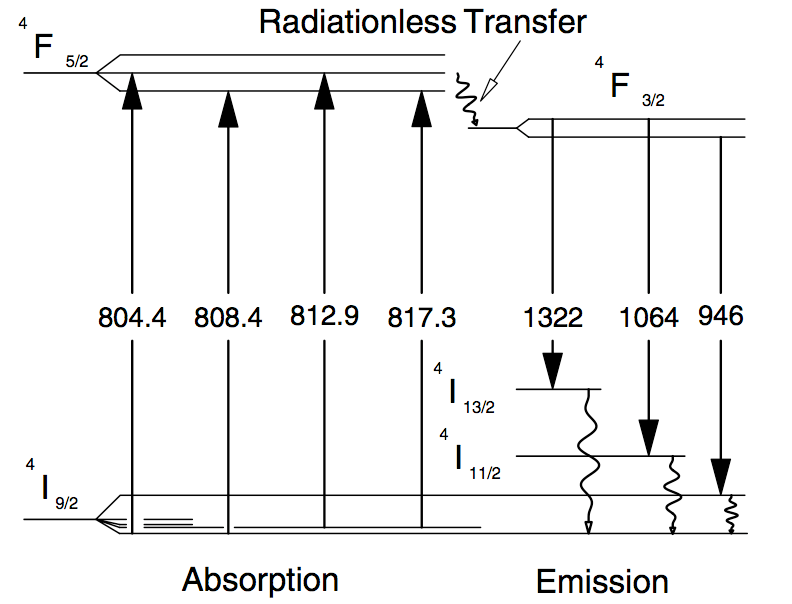
\includegraphics[width=0.5\textwidth]{img/termschema.png}
\caption{\small The term scheme for the Nd:YAG medium with the four-levels relevant for lasing. Taken from \cite{dickmann}}
\label{fig:termschema}
\end{figure}

\subsection{Resonator Geometry and Transversal Modes}
Resonators can be built as open or closed cavities. As the number of possible modes in a three dimensional confinement is large for achievable cavity sizes, one usually operates the laser in an open cavity formed by two mirrors, thus increasing the optical wave-length. At least one mirror is usually of finite curvature. The distance between the mirrors $L$ and the curvature radii $R_1$, $R_2$ determine the modes in the resonator. For one planar and one parabolic mirror (which is a good approximation for spherical mirrors of large radius), a criterion can be given for which modes can exist at all within the resonator as a consequence of the geometry and diffraction effects. This stability criterion is
\eq{ 0 < \lvert a- \frac{2L}{R} \rvert <1 \; ,}{stability}
where $L$ denotes the mirror distance and $R$ the curvature radius. The modes, which can be excited in such a resonator are given by 
\eq{\nu_p = \frac{c}{2L} \left[ p+1+\frac{1}{\pi}\arccos \left( 1-\frac{2L}{R}\right) \right] , } {modes}
where $p$ here denotes the order of the longitudinal mode (along the mirror-mirror-axis or $z$-axis) and $c$ is the velocity of light. The minimal distance between modes is then given by
\eq{\Delta \nu = \frac{c}{2L} .}{}
Additionally to the longitudinal modes, there are also transversal modes, which have also a component normal to the $z$-axis and are denoted with TEM (transversal electromagnetic mode). Their intensity profile in the $x-y$-plane is determined by the resonator geometry. For the special case of cylindrical and cartesian symmetries\footnote{More general solutions can be obtained by Ince-Gaussians \cite{ince}, that represent solutions for any elliptical geometry and include the special cases of Laguerre- and Hermite-Gaussians.}, the solution for the standing resonator waves are Laguerre-Gausians and Hermite-Gaussians respectively (cf.  fig. \ref{fig:modes}). For Laguerre-Gaussians, the modes are labeled TEM$_{rl}$, where $r$ and $l$ denote the radial and angular component (similar to spherical harmonics) and for Hermite-Gaussians TEM$_{nm}$ refer to the number of nodes in the two orthonormal directions within the plane normal to the $z$-axis.

\begin{figure}
\centering
\subfloat[][Hermite-Gaussians]{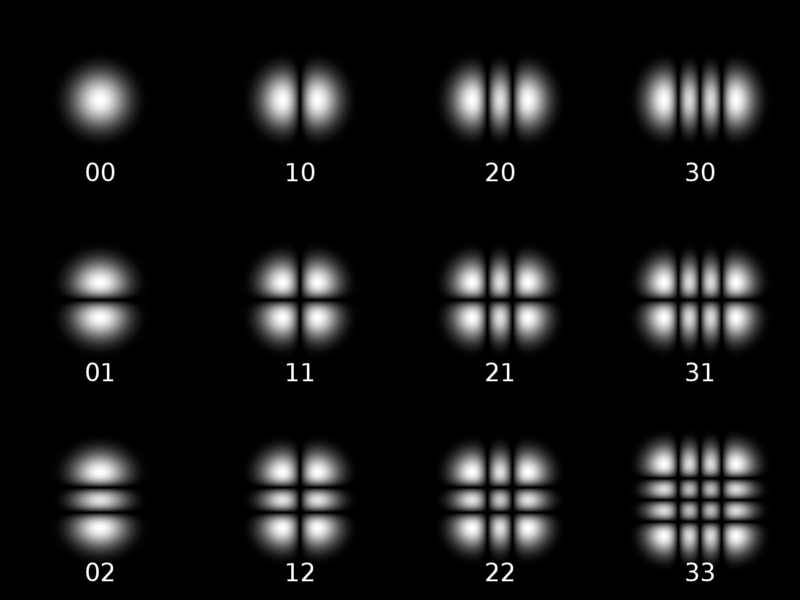
\includegraphics[width=0.48 \textwidth]{img/Hermite-gaussian.png}}
\hfill
\subfloat[][Laguerre-Gassuains]{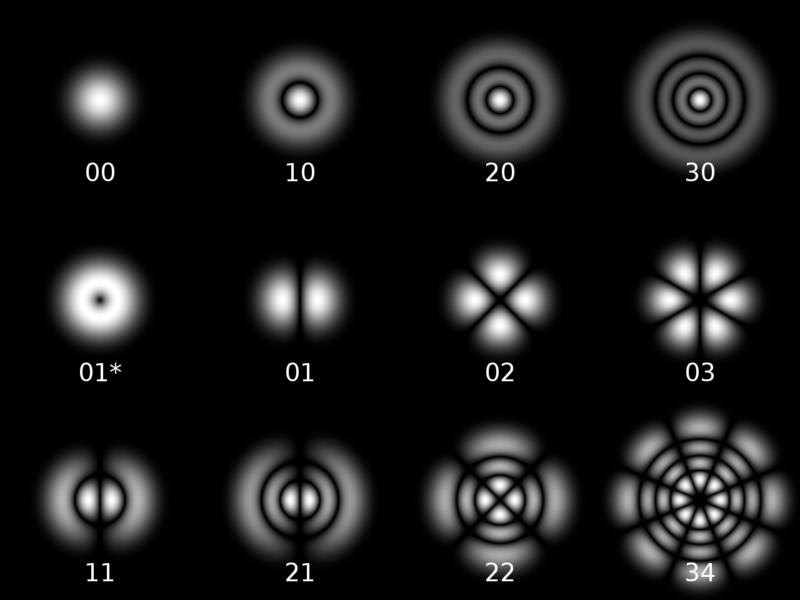
\includegraphics[width=0.48 \textwidth]{img/Laguerre-gaussian.png}}
\caption{\small Intensity profile within the plane normal to the laser beam for \textbf{(a)} cartesian and \textbf{(b)} cylindrical resonator geometries. Source: \url{http://en.wikipedia.org/wiki/Transverse_mode} }
\label{fig:modes}
\end{figure}

\subsection{Operating Figures of a Laser}
The general theory of the conditions for lasing were outlined in the previous sections. However, for experimental purposes some key figures of a laser are introduced to quantify the laser properties.

The lasing threshold describes the critical point, where pumping results in the emission of coherent light, i. e. the stimulated emission dominates the spontaneous emission. This coincides with the abrupt increase of laser light power with respect to pumping power. After threshold, the laser power increases linear with the pumping power (cf. fig. \ref{fig:threshold}), the proportionality coefficient $\Delta P$ is called slope efficiency and is given by
\eq{\Delta P = \frac{\Delta E_\text{laser}}{\Delta E_\text{pump}} \frac{T}{T+M} \; ,}{slope}
where $\Delta E_\text{laser}$ and $\Delta E_\text{pump}$ denote the energy of the laser relaxation and pumping excitation respectively, $T$ denotes the mirror transmission and $M$ the loss at the mirror. $\Phi$ is the quantum yield, which describes the percentage of incoming photons, which finally result in the desired process (here: the pumping transition). 

\begin{figure}
\centering
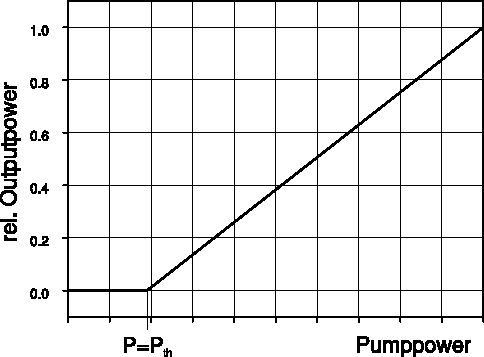
\includegraphics{img/threshold.pdf}
\caption{\small  Source: \cite{dickmann}}
\label{fig:threshold}
\end{figure}

\subsection{Diode Laser}
The pumping of the Nd:YAG laser is performed by an AlGaAs(Aluminium Galium Arsenid) diode laser, which provides the advantage of emission wavelengths, that can be tuned via the temperature and the  current through the diode. A further advantage is its compact form and the possibility to adjust the intensity via stack building. In this system a resonator is also only optional, because the solid state body itself acts as a resonator. The diode consists of a $p-n$-junction, which means, that an negatively and positively doped medium are brought into mechanical contact. The semi-conductor bandgap, can only be overcome if a voltage with correct sign is applied leading to recombination of electrons and holes, which are nothing but the lasing transition. It is the energy of the bandgap, which determines the wavelength of the emitted photons. As the population function of a solid state is influenced by temperature and voltage, this bandgap energy can thus be modulated.

\subsection{Pulsed Lasers}
For time resolved measurements or for measurements requiring high energies, pulses of laser light are preferable. The pulses can be generated by alternating the quality factor (Q-switching) of the resonator. This can be done passively, e.g. if the transmission of light happens only after the light intensity reaches a certain threshold or actively with opto-accustic cells like Pockels cells. Pockels cells consist of a crystal, which shows birefringence if external electric fields are applied. However in this case, the external magnetic field is aligned longitudinal or transversal to the light beam, which leads not to birefringence, but to a shift of polarization. If a polarization filter is inserted into the laser setup, this can then be used to alternate the quality factor of the resonator.

The repetition rate of the pulses can  be modulated via the Q-switching frequency, but the pulse duration $\Delta t$ is also influenced by the level of population inversion and the rate of its depletion. The minimal pulse duration is determined by the bandwidth product $\Delta \nu \Delta t$, where $\Delta \nu$ denotes the FWHM of the gain profile (cf. fig. \ref{gainprofile}) and $\Delta t$ the FWHM of the pulse profile. If both profiles are Gaussian shaped, the minimal product is limited by
\eq{\Delta \nu \Delta t > 0.44 \; .}{ftw}

The modulation of the modes inside the cavity can also result in an effect called mode locking. This term describes the in-phase alignment of different modes, which normally have a random phase distribution with respect to each other. Mode locking can occur, if the modulation with frequency $\nu_\text{mod}$ of one mode with frequency $\nu$ yields phase coherent higher order modes $\nu + \Delta \nu n$, match or a close to intrinsic laser modes. Those modes then also adapt the same phase as the mode $\nu$. 

\subsection{Nonlinear 
%o
Optics}
Nonlinear optics refers to the behavior of light in nonlinear media, i. e., media in which the dielectric polarization P responds nonlinearly to the electric field E of the light. This nonlinearity is typically only observed at very high light intensities, which can be achieved with pulsed lasers.
 
A prominent effect of nonlinear optics is the so called frequency doubling, which describes two photon at frequency $\nu$ creating a new single photon at frequency $2 \nu$. In this process energy conservation is obviously matched, but the conservation of momentum is critical due to the dispersion relation, which implies varying refractive indices at different frequencies. This however, can be managed by the use of a birefringent crystal. These crystals are singled out by a reduced symmetry compared to usual crystal, i.e. they poses only one symmetry axis, which is also called optical axis. The diffraction index for those crystals depends on the polarization (parallel or perpendicular with respect to the optical axis) and are called ordinary and extraordinary, where the extraordinary diffraction index depends on the incidence angle. Thus, with the right incidence angle $\Theta$ two differently polarized photon of different frequencies can pass the crystal at the same diffraction index (cf. fig \ref{fig:nonlinearofoptics}).

\begin{figure}
\centering
\subfloat[][Dispersion]{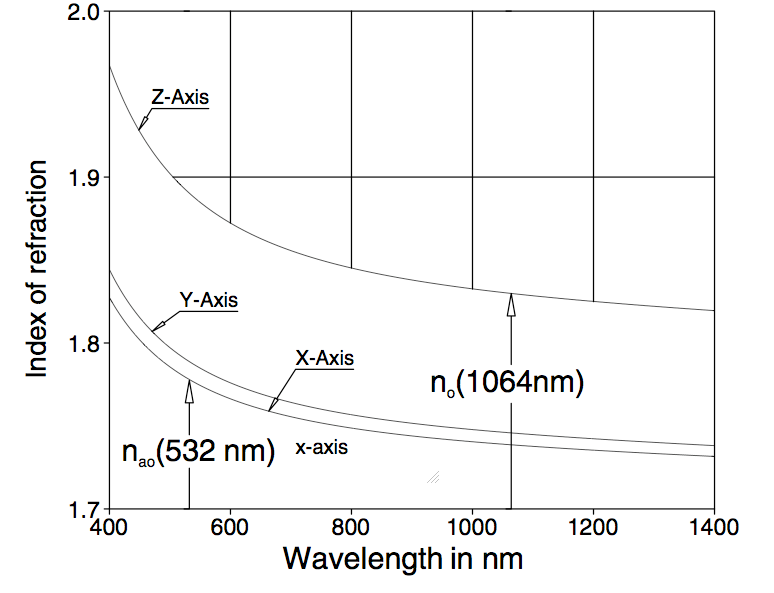
\includegraphics[width=0.45\textwidth]{img/nonlinearofoptics.png}}
\hfill
\subfloat[][Diffraction Ellipsoid]{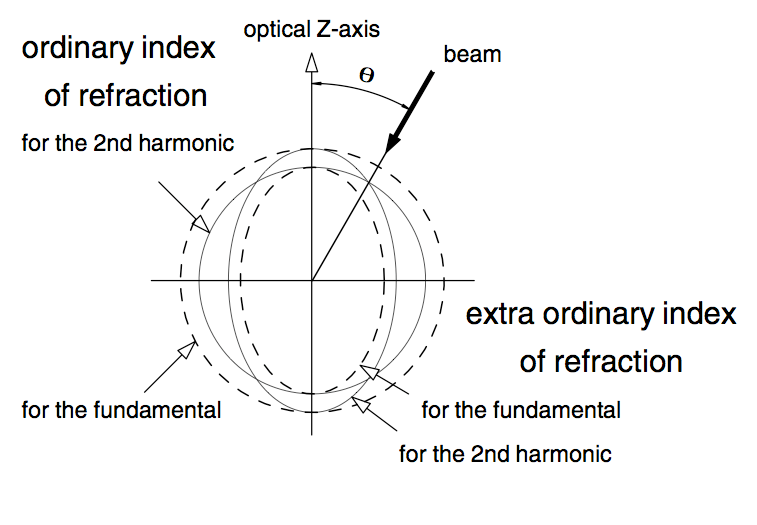
\includegraphics[width=0.45\textwidth]{img/ellips.png}}
\caption{\small \textbf{(a)} Dispersion relation in an anisotropic crystal. \textbf{(b)} Diffraction Index Ellipsoid for a birefringent crystal. Source : \cite{dickel}}
\label{fig:nonlinearofoptics}
\end{figure}

\section{Analysis}
\subsection{Pump Power of the Diode Laser}
The intensity spectrum of the light emitted from the diode laser depends on the temperature and on the current at which the diode is operated. In order to measure the power of the \SI{808.4}{nm} wavelength emission for varying currents, it has to be kept in mind, that that at a constant temperature, the wavelength will change with the current. Therefore the measurement was done for three different currents, for witch the exact temperature needed to provide \SI{808.4}{nm} emission is known from the calibration curves in \cite{script}. The linear dependency yields \eq{P_\text{diode}=\SI{1.05(1)}{\frac{mW}{mA}}\left(I_\text{diode}-\SI{160(1)}{mA} \right) \;, }{cal}
witch suggests a lasing threshold of about \SI{160(1)}{mA}. 




\subsection{Laser Parameters}
At \SI{34.4}{\degree C} the output power of the Nd:YAG was measured as a function of the laser diode current. Using the calibration of the previous measurement \Formel{cal} we obtain the output power as a function of the diode laser power. However, this measurement procedure does not take into account, that the wavelength of the diode laser changes with the current and also the total intensity. For the excitation of the active medium the wavelength of the pumping laser is crucial, but fortunately the pumping can be done not only at \SI{808.4}{nm}, but also at \SI{804.4}{nm} and thus it is expected, that the variations of the wavelength with the diode current is less dominant for the pumping efficiency then the changes in total intensity. To prove this and to further give an estimate about the error due to this assumption, a second measurement is performed, in which the dependence of the YAG power on temperature is investigated at a fixes current of \SI{500}{mA}. Within the measurement range of \SI{19}{ \degree C} to \SI{40}{\degree  C}, the emitted wavelength is expected to vary between \SI{804.3}{nm} and \SI{810.8}{nm}. In figure \ref{fig:temperature} it is clearly visible, that there is a broad plateau of the Nd:YAG intensity between \SI{21}{\degree C} and \SI{35}{\degree C} corresponding to the wavelengths \SI{804.9}{nm} and \SI{809.2}{nm} of the diode laser emission. This supports the hypothesis, that the ND:YAG medium is not too sensitive to wavelength changes as long as they do not exceed a certain range, that is roughly between \SI{805}{nm} and \SI{809}{nm}. From the calibration curves in \cite{script}, it can be said with some certainty, that this range is not exceeded in the measurement of the Nd:YAG power with respect to the diode laser current. Thus we conclude, that the calibration performed with \Formel{cal} is reliable enough to use it for qualitative calculations.

Considering the output-power vs. pump-power curve shown in figure \ref{fig:power}, the lasing threshold can be determined to be about $P_\text{thresh}=\SI{22(2)}{mW}$. Calculating the slope efficiency is more difficult, because the curve looks more like a saturation curve then like a linear line. It is likely, that either the power meter or the diode laser itself causes this effect. However, the slope efficiency can still be roughly estimated from a brutal linear fit to be $\Delta S = \SI{0.0147(4)}{}$.



\begin{figure}
\centering
\subfloat[][Diode Pump Power]{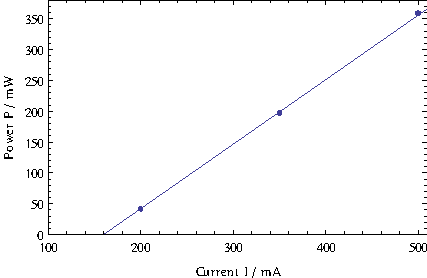
\includegraphics[width=0.485\textwidth]{img/PvsI808.pdf}}
\hfill
\subfloat[][Temperature Dependence]{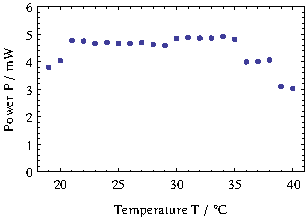
\includegraphics[width=0.485\textwidth]{img/temp.pdf}}
\caption{\small \textbf{(a)} Pump power of the diode laser for \SI{808.4}{nm} emission. The currents were measured at $36.3 \degree$ C, $34.4 \degree$ C and $32.4 \degree$ C (lower to higher currents). \textbf{(b)} Output Power of the Nd:YAG laser for different temperatures of the diode laser.}
\label{fig:nonlinearofoptics}
\end{figure}

\begin{figure}
\centering
\subfloat[][Diode Pump Power]{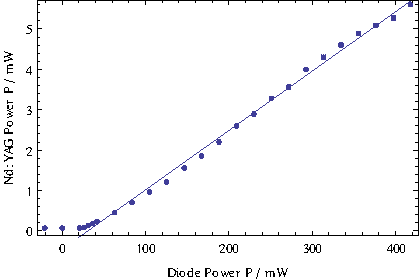
\includegraphics[width=0.485\textwidth]{img/totalegrade.pdf}}
\hfill
\subfloat[][Temperature Dependence]{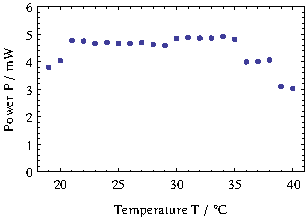
\includegraphics[width=0.485\textwidth]{img/temp.pdf}}
\caption{\small \textbf{(a)} Pump power of the diode laser for \SI{808.4}{nm} emission. The currents were measured at $36.3 \degree$ C, $34.4 \degree$ C and $32.4 \degree$ C (lower to higher currents). \textbf{(b)} Output Power of the Nd:YAG laser for different temperatures of the diode laser.}
\label{fig:nonlinearofoptics}
\end{figure}








\clearpage
 \bibliographystyle{unsrt}
\bibliography{bib}











\end{document}